\section{Motivating Example}

As a motivating example, imagine a user was to reconstruct the filter that was used to transform an audio clip, as shown in Figure~\ref{fig:test}.
In this example, a user provided a clip of a \texttt{cartoon-spring.wav} in Figure~\ref{fig:inEx}, and the same sound as it had been transformed with a low-pass filter at 800 Hz, $lpf(800)$, as shown in Figure~\ref{fig:outEx}.
However the nature of the transformation is unknown to the user and they wish to discover the filter needed.
Our DSP-PBE tool is able to synthesize a filter $lpf(1989)$, that when applied to the original sound, produces the waveform shown in Figure~\ref{fig:synthEx}.
While the solution is not exact, the difference is not significantly noticeable to an untrained ear.

\begin{figure}
\centering
\begin{subfigure}{.32\linewidth}
  \centering
  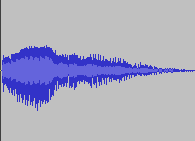
\includegraphics[width=.9\textwidth]{figs/original.png}
  \caption{Input example}
  \label{fig:inEx}
\end{subfigure}%
\begin{subfigure}{.32\linewidth}
  \centering
  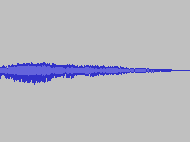
\includegraphics[width=.9\textwidth]{figs/lpf800.png}
  \caption{Output example}
  \label{fig:outEx}
\end{subfigure}
\begin{subfigure}{.32\linewidth}
  \centering
  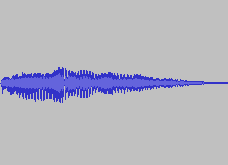
\includegraphics[width=.9\textwidth]{figs/lpf1989.png}
  \caption{Generated}
  \label{fig:synthEx}
\end{subfigure}
\caption{The waveforms (a) and (b) are provided as examples, and DSP-PBE synthesizes a filter that produces (c).}
\label{fig:test}
\end{figure}

